\documentclass[a4paper,11pt]{article}
%Premeable
	%Chinese
	\usepackage[UTF8,fontset=fandol]{ctex}
	\usepackage{xeCJK}
	\usepackage[datesep=/]{datetime2}
	\DeclareTextFontCommand{\textbf}{\sffamily}
%Presenting
	\usepackage[table]{xcolor}
	\usepackage{graphicx}
	\usepackage[font={sf}]{caption}
	\usepackage[above]{placeins}
	\usepackage{float,wrapfig}
	\usepackage{tabularx,array,booktabs,multirow,bigstrut}
	\newcolumntype{C}[1]{>{\hsize=#1\hsize%
		\centering\arraybackslash}X}
	\newcommand{\minitab}[2][l]{%
		\begin{tabular}{#1}#2\end{tabular}}
%MathSetting
	\let\latexointop\ointop
	\usepackage{amsmath,bm,amssymb,esint,extarrows}
	\usepackage{upgreek,textcomp,mathrsfs}
	\usepackage[only,sslash]{stmaryrd}
	\usepackage{nicefrac,eqnarray}
%	\usepackage{amsthm}
	\usepackage{mathtools,physics,siunitx}
	\usepackage{stackengine,titling,varwidth}
	\usepackage{tikz}
	\usepackage{resizegather,empheq}
	\usetagform{default}
	\usepackage{calligra,fourier-orns}
	% Keep \oint unchanged by esint
	\let\ointop\undefined
	\let\ointop\latexointop
	% Define a scriptr 
	\DeclareMathAlphabet{\mathcalligra}{T1}{calligra}{m}{n}
	\DeclareFontShape{T1}{calligra}{m}{n}{<->s*[2.2]callig15}{}
	\newcommand{\scriptr}{\mathcalligra{r}\,}
	\newcommand{\rvector}{\pmb{\mathcalligra{r}}\,}
	% Useful shorthand
	\DeclarePairedDelimiter\ave{\langle}{\rangle}
	\newcommand\inlineeqno{\stepcounter{equation}\ (\theequation)}
	\newcommand{\sinc}{\operatorname{sinc}}
	\newcommand{\mbb}[1]{\mathbb{#1}}
	\newcommand{\mrm}[1]{\mathrm{#1}}
	\newcommand{\mcal}[1]{\mathcal{#1}}
	% Scaling and positioning
	\newcommand\scalemath[2]{\scalebox{#1}{\mbox{\ensuremath{\displaystyle #2}}}}
	\newcommand\raisemath[2]{\raisebox{#1\depth}{${#2}$}}
	\empheqset{box=\bbox}
	% Presenting
	\newcommand*\bbox[1]{\fbox{\hspace{1em}\addstackgap[5pt]{#1}\hspace{1em}}}
	\sisetup{%
		redefine-symbols=false,%
		separate-uncertainty=true,%
		range-phrase=\,\textasciitilde\,,%
		arc-separator = \,}
	\allowdisplaybreaks[2]
%ParagraphSetting
	\setlength{\parskip}{.3\baselineskip}
	\usepackage[defaultlines=2,all]{nowidow}
	\postdisplaypenalty=50
%PageSetting
	\usepackage[colorlinks=true,linkcolor=blue]{hyperref}
	\usepackage[vmargin={4cm,5cm},hmargin=3cm,%
		footnotesep=\baselineskip]{geometry}
	\usepackage[bottom]{footmisc}
	\usepackage{changepage}
	% Autoref names
	\renewcommand{\tableautorefname}{\tablename}
	\renewcommand{\figureautorefname}{\figurename}
	% List settings
	\usepackage{enumitem}
	\setlist{itemsep=0pt,topsep=0pt,labelindent=\parindent,leftmargin=0pt,itemindent=*}
	% Some redefined lengths
	\setlength{\headsep}{2.2cm}
	\setlength{\droptitle}{-2.2cm}
	\setlength{\footnotesep}{3\parskip}
	% Header
	\usepackage{fancyhdr,lastpage}
	\pagestyle{fancy}
	\fancyhf{}
	\cfoot{--\ \thepage\,/\,\pageref{LastPage} \ --}
	\renewcommand{\headrulewidth}{0.1pt}
	\renewcommand{\headrule}{
		\vbox to 2pt{
		\hbox to \headwidth{\dotfill}\vss}}
	% Separator
	\newcommand{\newparagraph}{\pagebreak[3]\noindent%
		\hfil
		~\raisebox{-4pt}[10pt][10pt]{\decofourright~~~~~~~~\decofourleft}~ %
		\par
	}
%TitleSettings
	\pretitle{\begin{center}}
	\posttitle{\par\end{center}\vspace{-6mm}}
	\predate{}
	\postdate{\vspace{-4mm}}
%Header
	\lhead{%
		
\includegraphics[height=3.2em]{PKUPhy.png}
		\vspace{-3ex}
		}
	\rhead{%
		\itshape\small
		\begin{tabular}{rr}
			\multicolumn{2}{r}{赵启渊} \\[.3em]
			学号:   & 2000011153 \\[.2em]
		\end{tabular}\hspace{-1em}
		}
%Title
	\title{\textit{\large 实验七}\\[2mm]
		\textbf{\LARGE 测量误差和数据处理}}
	\author{\textit{赵启渊} 2000011153}
	\date{}
%Miscellaneous
	\newcommand{\tabindent}{\hspace{2em}}
%FourierTransform
	\newcommand{\ftransform}{\xlongrightarrow{\ \mathscr F\ }}
	\newcommand{\iftransform}{\xlongrightarrow{\ \mathscr F^{-1}\ }}
	\usepackage{gensymb}

\begin{document}
	\vspace*{1cm}
	
	\vspace*{1cm}
	
	\begin{center}
		\Huge{\textbf{基础物理实验报告}}
		
		\Large{测量误差和数据处理}
	\end{center}
	
	\vspace*{2cm}
	
	\begin{table}[h]
		\centering	
		\begin{Large}
			\begin{tabular}{p{3cm} p{7cm}<{\centering}}
				姓\qquad 名: & 赵启渊 \\
				\hline
				学\qquad 院: & 工学院 \\
				\hline
				学\qquad 号: & 2000011153 \\
				\hline
				分\qquad 组: & 第1组7号 \\
				\hline
				日\qquad 期: & 2022年3月23日 \\
				\hline
				指导教师: & 刘春玲\ 张艳席\\
				\hline
			\end{tabular}
		\end{Large}
	\end{table}
	
\maketitle
\thispagestyle{fancy}
\section{数据及处理}
\subsection{测量钢杯含钢体积}
	用允差为0.02mm的游标卡尺测量钢杯的外径D、内径d、高H、深h,测定数据并进行修正和不确定度的计算,测定数据及结果如下:
	
	\begin{table}[H]
	\centering\caption{测量钢杯含钢体积的数据表}
	\small
	\begin{tabularx}{.85\linewidth}{C{1} *6{C{.8}}}
	\toprule
		\textbf{项目} &
		$D / \si{\cm}$ &
		$d / \si{\cm}$ &
		$h / \si{\cm}$ &
		$H / \si{\cm}$ & \\
	\midrule
	    读数零点     & 0.002  & 0.002  & 0.002 & 0.002 &   \\
		1     & 2.810  & 1.988  & 3.202 & 4.520    &  \\
		2     & 2.820  & 1.996  & 3.230 & 4.530    &   \\
		3     & 2.818  & 1.992  & 3.240 & 4.518    &  \\
		4     & 2.812  & 1.994  & 3.208 & 4.514    &  \\
		5     & 2.818  & 1.970  & 3.210 & 4.518    &  \\
		6     & 2.816  & 1.984  & 3.214 & 4.516    &  \\
		平均值    & 2.8157  & 1.987  & 3.217 & 4.5193 & \\
		平均值的标准差     & 0.0016  & 0.004  & 0.006 & 0.0023 &\\
		考虑仪器允差之后的标准差     & 0.0020  & 0.004  & 0.006 & 0.0026  &\\
		修正零点后的平均值     & 2.8137  & 1.985  & 3.215 & 4.5173 &\\
		
	\bottomrule
	\end{tabularx}
	\vspace{3ex}
	\end{table}\noindent%
    其中平均值的标准差计算使用$$ \sqrt{\frac{\sum _{j=1}^{n}{\left({N}_{j}-\stackrel{-}{N}\right)}^{2}}{n\left(n-1\right)}} $$
	考虑仪器允差之后的标准差计算使用$$\sqrt{\frac{\sum _{j=1}^{n}{\left({N}_{j}-\stackrel{-}{N}\right)}^{2}}{n\left(n-1\right)}+{\left(\frac{e}{\sqrt{3}}\right)}^{2}}$$
    平均值零点修正计算使用$$\stackrel{-}{N}-{N}_{0}$$
    \begin{enumerate}
    	\item 测量结果: 
    	$$\stackrel{-}{D} ± \sigma_{D} = (2.8137 ± 0.0020) cm$$
    	$$\stackrel{-}{d} ± \sigma_{d} = (1.985 ± 0.004) cm$$
    	$$\stackrel{-}{h} ± \sigma_{H} = (3.215 ± 0.006) cm$$
    	$$\stackrel{-}{H} ± \sigma_{h} = (4.5173 ± 0.0026) cm$$
    	\item 计算结果:
    	$$V = \dfrac{\pi}{4} * ( \stackrel{-}{D}^{2} * \stackrel{-}{H} - \stackrel{-}{d}^{2} * \stackrel{-}{h} ) =  18.14  cm^{3}$$
    	$$ \sigma_{V} = \sqrt{(\dfrac{\partial V}{\partial D} * \sigma_{D})^{2} + (\dfrac{\partial V}{\partial d} * \sigma_{d})^{2} + (\dfrac{\partial V}{\partial H} * \sigma_{H})^{2} + (\dfrac{\partial V}{\partial h} * \sigma_{h})^{2} } $$
    	$$ = \sqrt{(\dfrac{\pi}{2} * D * H *\sigma_{D} )^{2} + (- \dfrac{\pi}{2} * d * h *\sigma_{d} )^{2} + (\dfrac{\pi}{4} * D^{2}*\sigma_{H} )^{2} + (- \dfrac{\pi}{4} *  d^{2} *\sigma_{h} )^{2}} $$
    	$$ = 0.06 cm^{3}$$
    	$$ V ± \sigma_{V} = ( 18.14 ± 0.06 ) cm^{3} $$
    \end{enumerate}
	
\subsection{测量小钢球体积}
	用允差为0.004mm的螺旋测微器测量小钢球直径d,并计算其结果的不确定度, 测定数据及结果如下:
	
	\begin{table}[H]
		\centering\caption{测量小钢球体积的数据表}
		\small
		\begin{tabularx}{.85\linewidth}{C{1} *6{C{.8}}}
			\toprule
			\textbf{项目} &
			$d / \si{\cm}$ &\\
			\midrule
			读数零点     & 0.0000  &   \\
			1     & 1.2696  &   \\
			2     & 1.2697  &   \\
			3     & 1.2698  &   \\
			4     & 1.2695  &   \\
			5     & 1.2696  &   \\
			6     & 1.2697  &   \\
			平均值    & 1.26965  & \\
			平均值的标准差     & 0.00004  & \\
			考虑仪器允差之后的标准差     & 0.00023  & \\
			修正零点后的平均值     & 1.26965  & \\
			
			\bottomrule
		\end{tabularx}
		\vspace{3ex}
	\end{table}\noindent%

    其中平均值的标准差计算使用$$ \sqrt{\frac{\sum _{j=1}^{n}{\left({N}_{j}-\stackrel{-}{N}\right)}^{2}}{n\left(n-1\right)}} $$
    考虑仪器允差之后的标准差计算使用$$\sqrt{\frac{\sum _{j=}^{n}{\left({N}_{j}-\stackrel{-}{N}\right)}^{2}}{n\left(n-1\right)}+{\left(\frac{e}{\sqrt{3}}\right)}^{2}}$$
    平均值零点修正计算使用$$\stackrel{-}{N}-{N}_{0}$$
    
    \begin{enumerate}
    	\item 测量结果: 
    	$$\stackrel{-}{d} ± \sigma_{d} = (1.26965 ± 0.00023) cm$$
    	\item 计算结果:
    	$$V = \dfrac{\pi}{6} * \stackrel{-}{d}^{3} =  1.0716  cm^{3}$$
    	$$ \sigma_{V} = \sqrt{(\dfrac{\partial V}{\partial d} * \sigma_{d})^{2} } $$
    	$$ = \sqrt{(\dfrac{\pi}{2} * d^{2} *\sigma_{d} )^{2} } $$
    	$$ = 0.0006 cm^{3}$$
    	$$ V ± \sigma_{V} = ( 1.0716 ± 0.0006 ) cm^{3} $$
    \end{enumerate}
	
	
\section{习题:}
\ \\
1.\\ 

(1) 1位有效数字。\ (2) 4位有效数字。\ (3) 2位有效数字。\ (4) 6位有效数字。\\
2.\\

(1)$$ c=\dfrac{1}{\frac{1}{a} - \frac{1}{b}} = 10 cm $$

(2)$$ -x^{2} = - 85.3 $$
$$ y = e^{- 85.3} = 9 * 10^{-38} $$

(3)$$ y = \ln(x) = 4.038 $$

(4)$$ y = \cos(x) = 0.99$$
3.\\

(b)$$ \sigma_{\rho} = \sqrt{(\dfrac{\partial \rho}{\partial m_{1}} * \sigma_{m_{1}})^{2} + (\dfrac{\partial \rho}{\partial m_{2}} * \sigma_{m_{2}})^{2}  } $$
$$ = \rho_{0}*\sqrt{(- \dfrac{m_{2}}{(m_{1}-m_{2})^{2}} * \sigma_{m_{1}})^{2} + (\dfrac{m_{1}}{(m_{1}-m_{2})^{2}} * \sigma_{m_{2}})^{2}  }$$
$$ = \dfrac{\rho_{0}}{(m_{1}-m_{2})^{2}}*\sqrt{({m_{2}} * \sigma_{m_{1}})^{2} + ( {m_{1}}  * \sigma_{m_{2}})^{2}  }$$

(c)$$ \sigma_{y} = \sqrt{(\dfrac{\partial y}{\partial a} * \sigma_{a})^{2} + (\dfrac{\partial y}{\partial b} * \sigma_{b})^{2}  } $$
$$  = \sqrt{(\dfrac{b}{a * ( a + b )} * \sigma_{a})^{2} + (\dfrac{a}{b * ( a + b )} * \sigma_{b})^{2}  } $$
$$  = \dfrac{1}{a + b}*\sqrt{(\dfrac{b}{a} * \sigma_{a})^{2} + (\dfrac{a}{b} * \sigma_{b})^{2}  } $$
4.\\

最合理的方法是只测$L_{1}$和$L_{2}$的长度,这样就有$$L = \frac{1}{2}*(L_{1} + L_{2})$$
5.\\
$$ \dfrac{\sigma_{S}}{N} = \sqrt{(\dfrac{\partial \ln(S)}{\partial L_{1}} * \sigma_{L_{1}})^{2} + (\dfrac{\partial \ln(S)}{\partial L_{2}} * \sigma_{L_{2}})^{2} + (\dfrac{\partial \ln(S)}{\partial d_{1}} * \sigma_{d_{1}})^{2} + (\dfrac{\partial \ln(S)}{\partial d_{2}} * \sigma_{d_{2}})^{2} } $$
$$ = \dfrac{1}{L_{1}*L_{2} - \frac{\pi}{4} * d_{1}^{2} - \frac{\pi}{4} * d_{2}^{2}}\sqrt{(L_{2} * \sigma_{L_{1}})^{2} + (L_{1} * \sigma_{L_{2}})^{2} + (\dfrac{\pi}{2} * d_{1}* \sigma_{d_{1}})^{2} + (\dfrac{\pi}{2} *d_{2} * \sigma_{d_{2}})^{2} } $$
由题意知
$$ \dfrac{\sigma_{S}}{N} <= 0.5\% $$
得到$$ \sigma_{d_{2}} <= 1.156 $$
因为$ d_{2} >= \sigma_{d_{2}} $, 所以题中测量的$ \sigma_{d_{2}} $一定要比极端情况下的不确定度小,因此使用题中测量$ d_{2}  $的方法就可以满足题意。  \\
7.\\

(1)$$ g_{0} = \dfrac{2*h_{0}}{t_{0}^{2}}$$
$$ g = \dfrac{2*h}{t^{2}}$$
$$ = \dfrac{2*h_{0}*(1+10^{-4})}{t_{0}^{2}*(1-10^{-4})^{2}} $$
$$ = g_{0} * 1.0003 $$
$$ = 980.3 cm/s^{2} $$

(2)\\
因为四次项展开的影响因素过小,因此考虑它的二次项展开:
$$ \frac{1}{4} * \sin[2](\frac{\theta}{2}) <= 0.5 \%$$
$$ \frac{\theta}{2} <= 8.13 \degree $$
$$ \theta <= 16.3 \degree $$
同理得
$$ \frac{1}{4} * \sin[2](\frac{\theta}{2}) <= 0.05 \%$$
$$ \frac{\theta}{2} <= 2.56 \degree $$
$$ \theta <= 5.12 \degree $$

10.\\
$$\lambda = \dfrac{6}{k*(k+2)*d}*(2*\stackrel{-}{y_{i}}-k*\stackrel{-}{y}) $$
这里$k=9$ \  $ d=1 $
$$\stackrel{-}{y_{i}} = \frac{1}{10}\sum _{j=0}^{9}j{y}_{j} = 373.0679 $$
$$\stackrel{-}{y} = 66.8571 $$
因此$$ \lambda = 8.753  mm$$
$$ c = f * \lambda = 346.4 m/s$$
计算不确定度:\\
$$ c=\lambda * f $$
$$ \ln(c)=\ln(\lambda) * \ln(f) $$
对表达式求微分得:
$$ \frac{\mathrm{d}c}{c} = \frac{\mathrm{d}f}{f} + \frac{\mathrm{d}\lambda}{\lambda}$$
$$ \frac{\sigma_{c}}{c} = \sqrt{(\frac{\sigma_{f}}{f})^{2} + (\frac{\sigma_{\lambda}}{\lambda})^{2}} $$
$ \sigma_{\lambda} $由随机误差和系统误差组成,随机误差:
$$ \sigma_{\lambda1} = \lambda * \sqrt{\dfrac{\frac{1}{r^{2}}-1}{n-2}}$$
$$ r = \dfrac{\sum _{i=1}^{10}(x_{i} - \stackrel{-}{x})*(y_{i} - \stackrel{-}{y})}{\sqrt{\sum _{i=1}^{10}(x_{i} - \stackrel{-}{x})^{2} * \sum _{i=1}^{10}(y_{i} - \stackrel{-}{y})^{2}}} = 0.999969 $$
系统误差:
$$ \sigma_{\lambda2} = \dfrac{\frac{e_{1}}{\sqrt{3}}}{\sqrt{\sum _{i=1}^{10}(x_{i} - \stackrel{-}{x})^{2}}} $$
$$e_{1}= 0.005$$
$$ \sigma_{\lambda3} = \dfrac{\frac{e_{2}}{\sqrt{3}}}{\sqrt{\sum _{i=1}^{10}(x_{i} - \stackrel{-}{x})^{2}}} $$
$$e_{2}= 0.01$$
合成
$$\sigma_{\lambda}^{2} = \sigma_{\lambda1}^{2} +\sigma_{\lambda2}^{2} + \sigma_{\lambda3}^{2} =  6.544 * 10^{-4}$$
又因为:
$$\sigma_{f} = \frac{e_{f}}{\sqrt{3}} $$
所以:$$ \sigma_{c} = 1.0 m/s $$
11.\\

(1)\begin{figure}[H]
	\centering
	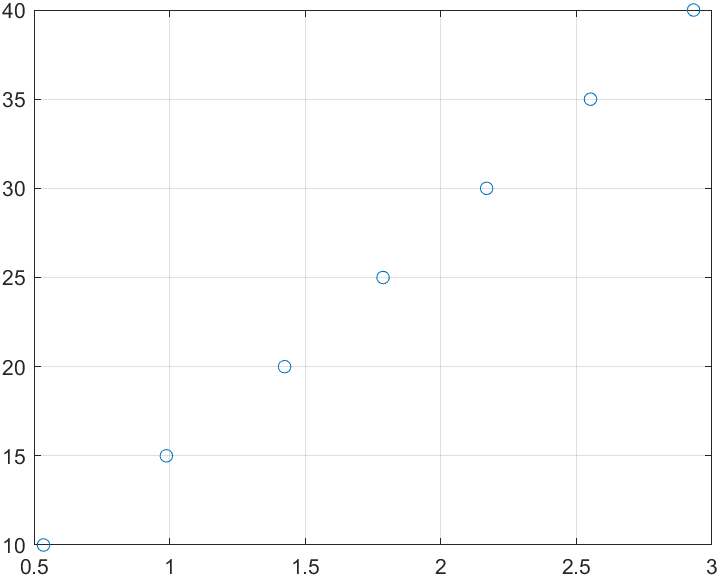
\includegraphics[width=.6\linewidth]{line1.png}
	\caption{刚体转动实验线性回归图}
\end{figure}\noindent%
由图可知$m-\frac{1}{t^{2}}$是线性关系。

(2)令$ x=m \ y=\frac{1}{t^{2}} $
$$ k_{2} = \dfrac{\sum _{i=1}^{7}(x_{i} - \stackrel{-}{x})*(y_{i} - \stackrel{-}{y})}{\sum _{i=1}^{7}(x_{i} - \stackrel{-}{x})^{2}} $$
$$ \stackrel{-}{y} = 1.770 $$
$$ \stackrel{-}{x} = 25 $$
$$ k_{2} = 0.079 $$
$$ b_{2} = \stackrel{-}{y} - k_{2}*\stackrel{-}{x} = -0.206 $$
$$ r_{2} = \dfrac{\sum _{i=1}^{7}(x_{i} - \stackrel{-}{x})*(y_{i} - \stackrel{-}{y})}{\sqrt{\sum _{i=1}^{7}(x_{i} - \stackrel{-}{x})^{2} * \sum _{i=1}^{7}(y_{i} - \stackrel{-}{y})^{2}}} = 0.99933 $$

(3)令$ x=\frac{1}{t^{2}} \ y=m $
$$ k_{1} = \dfrac{\sum _{i=1}^{7}(x_{i} - \stackrel{-}{x})*(y_{i} - \stackrel{-}{y})}{\sum _{i=1}^{7}(x_{i} - \stackrel{-}{x})^{2}} $$
$$ \stackrel{-}{y} = 25 $$
$$ \stackrel{-}{x} = 1.770 $$
$$ k_{1} = 12.637 $$
$$ b_{1} = \stackrel{-}{y} - k_{2}*\stackrel{-}{x} = 2.638 $$
$$ r_{1} = \dfrac{\sum _{i=1}^{7}(x_{i} - \stackrel{-}{x})*(y_{i} - \stackrel{-}{y})}{\sqrt{\sum _{i=1}^{7}(x_{i} - \stackrel{-}{x})^{2} * \sum _{i=1}^{7}(y_{i} - \stackrel{-}{y})^{2}}} = 0.99933 $$
由计算结果有
$$r_{1}=r_{2}$$
因为在相关系数的计算中,x 与 y的关系是等价的,即x与y可以调换而不影响结果。因此将自变量应变量调换之后,不影响r的计算。\\
由计算公式有
$$r_{1}=r_{2}= \sqrt{k_{1}*k_{2}}$$



\section{分析与讨论}
\subsection{关于钢杯体积不确定度的进一步分析}
$$ \sigma_{V} = \sqrt{(\dfrac{\partial V}{\partial D} * \sigma_{D})^{2} + (\dfrac{\partial V}{\partial d} * \sigma_{d})^{2} + (\dfrac{\partial V}{\partial H} * \sigma_{H})^{2} + (\dfrac{\partial V}{\partial h} * \sigma_{h})^{2} } $$
$$ = \sqrt{(\dfrac{\pi}{2} * D * H *\sigma_{D} )^{2} + (- \dfrac{\pi}{2} * d * h *\sigma_{d} )^{2} + (\dfrac{\pi}{4} * D^{2}*\sigma_{H} )^{2} + (- \dfrac{\pi}{4} *  d^{2} *\sigma_{h} )^{2}} $$
由随机误差带来的不确定度
$$ \sqrt{(\dfrac{\pi}{2} * D * H *\sigma_{\stackrel{-}{D}} )^{2}  + (- \dfrac{\pi}{2} * d * h *\sigma_{\stackrel{-}{d}} )^{2} + (\dfrac{\pi}{4} * D^{2} *\sigma_{\stackrel{-}{H}} )^{2}  + (- \dfrac{\pi}{4} *  d^{2} *\sigma_{\stackrel{-}{h}} )^{2} }  $$
$$ = \sqrt{3.24*10^{-3}}  $$
由系统误差带来的不确定度
$$ \sqrt{(\dfrac{\pi}{2} * D * H *\frac{e_{D}}{\sqrt{3}} )^{2} + (- \dfrac{\pi}{2} * d * h *\frac{e_{d}}{\sqrt{3}} )^{2} + (\dfrac{\pi}{4} * D^{2}*\frac{e_{H}}{\sqrt{3}} )^{2} + (- \dfrac{\pi}{4} *  d^{2} *\frac{e_{h}}{\sqrt{3}} )^{2}}  $$
$$= \sqrt{7.30*10^{-4}}$$
由数据可以看出:随机误差带来的不确定度大。
	
\subsection{关于小钢球体积不确定度的进一步分析}
$$ \sigma_{V} = \sqrt{(\dfrac{\partial V}{\partial d} * \sigma_{d} )^{2} } $$
$$ = \sqrt{(\dfrac{\pi}{2} * d^{2} *\sigma_{d} )^{2} } $$
由随机误差带来的不确定度
$$ \sqrt{(\dfrac{\partial V}{\partial d} * \sigma_{\stackrel{-}{d}})^{2} }  $$
由系统误差带来的不确定度
$$ \sqrt{(\dfrac{\partial V}{\partial d} * \frac{e_{h}}{\sqrt{3}} )^{2} }  $$
因此只需要比较$\sigma_{\stackrel{-}{d}}$与$\frac{e_{h}}{\sqrt{3}}$的大小即可。
$$ \sigma_{\stackrel{-}{d}} = 0.00004 $$
$$ \frac{e_{h}}{\sqrt{3}} = 0.00023 $$
由数据可以看出:系统误差带来的不确定度大。
	
\section{收获与感想}
\subsection{灵活减少数据不确定度}
	由上述分析可见,在不同的实验中,系统误差和随机误差对于结果不确定度的影响是不同的,对于随机误差带来不确定度大的情况,应该增加测量次数,以降低其影响;对于系统误差带来不确定度大的情况,应该改进实验步骤或者使用更加精密的测量仪器来进行实验。还要结合实验实际,尽可能降低实验已定系统误差的影响。
\subsection{有效数字的运算规则}
	\begin{enumerate}
		\item 先按小数点后位数最少的数据保留其它各数的位数,再进行加减计算,计算结果也使小数点后保留相同的位数。
		\item 先按有效数字最少的数据保留其它各数,再进行乘除运算,计算结果仍保留相同有效数字。
		\item 乘方开方运算中,结果的有效数字和底数有效数字相同。
		\item 对数计算中,结果中尾数的有效数字位数和真数有效数字位数相同。
		\item 指数计算中,结果有效数字的位数和指数小数点后的有效数字位数相同(包括紧接着小数点后面的0)
		\item 三角函数的有效数字位数和角度的有效数字位数相同。
	\end{enumerate}

\subsection{有效数字的书写规则}
\begin{enumerate}
	\item 在直接测量一次的情况下,测量结果的有效数字最后一位要与仪器允差或估计的不确定度的最后一位取齐。
	\item 在多次直接测量求算术平均值的情况下,先计算算术平均值的不确定度,将算术平均值有效数字的最后一位与不确定度的最后一位取齐。
	\item 在间接测量结果的情况下,先计算间接测量结果的不确定度,将间接测量结果有效数字的最后一位与不确定度的最后一位取齐。
\end{enumerate}

	\vfill\noindent\itshape\footnotesize
	\hfill Last edited: \today\ \copyright\ 赵启渊
\end{document}